% 2007 年四川卷理科第 4 题：正方体 ABCD-A_1B_1C_1D_1 及两条面对角线、两条体对角线。
% 来源 PDF：gaokaomath-src/普通高考/2007/2007四川理.pdf，SHA256 6f3287a6ec1c136fb7e457cb0264d069c44eb8ff58a81cc3598f9c8f1395cc2d
% 原页：2007四川理.pdf 第 1 页（A3 三栏）第 1 栏，书页码 409，图在第 4 题题干下方。
% 重绘依据：斜投影画法，前面 ABB_1A_1 为正方形（A 左下、B 右下、A_1 左上、B_1 右上），
%   棱长方向 (1,0)、高方向 (0,1)，纵深方向取 (0.5,0.3)（D_1 在 A_1 右上方）；
%   可见棱 A_1B_1、B_1C_1、C_1D_1、D_1A_1、A_1A、B_1B、C_1C、AB、BC 与可见辅助线
%   B_1D_1、B_1C 画实线；不可见棱 AD、DC、DD_1 与辅助线 BD、D_1B、D_1C、AC_1 画虚线。
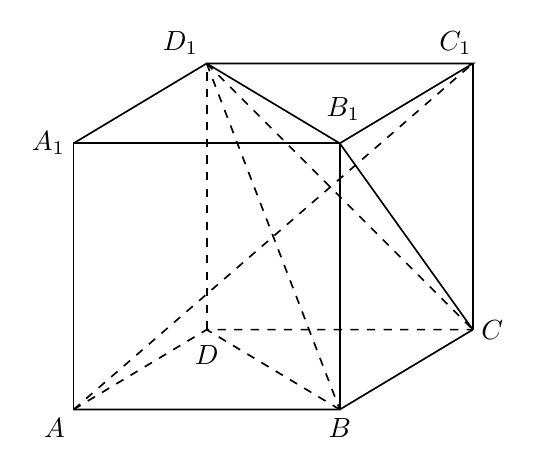
\begin{tikzpicture}[scale=1.3, semithick,
  every node/.style={inner sep=1.5pt}]
  \coordinate (A)  at (0,0);
  \coordinate (B)  at (2.6,0);
  \coordinate (A1) at (0,2.6);
  \coordinate (B1) at (2.6,2.6);
  \coordinate (D)  at (1.3,0.78);
  \coordinate (C)  at (3.9,0.78);
  \coordinate (D1) at (1.3,3.38);
  \coordinate (C1) at (3.9,3.38);
  % 不可见棱与不可见辅助线
  \draw[dashed] (A) -- (D) -- (C);
  \draw[dashed] (D) -- (D1);
  \draw[dashed] (B) -- (D);
  \draw[dashed] (D1) -- (B);
  \draw[dashed] (D1) -- (C);
  \draw[dashed] (A) -- (C1);
  % 可见棱
  \draw (A) -- (B) -- (C);
  \draw (A) -- (A1) -- (B1) -- (B);
  \draw (A1) -- (D1) -- (C1) -- (B1);
  \draw (C) -- (C1);
  % 可见辅助线
  \draw (B1) -- (D1);
  \draw (B1) -- (C);
  \node[anchor=north east] at ([xshift=-1pt,yshift=-1pt]A) {$A$};
  \node[anchor=north] at ([yshift=-1pt]B) {$B$};
  \node[anchor=west] at ([xshift=1pt]C) {$C$};
  \node[anchor=north] at ([yshift=-3pt]D) {$D$};
  \node[anchor=east] at ([xshift=-1pt]A1) {$A_1$};
  \node[anchor=south] at ([xshift=1pt,yshift=5pt]B1) {$B_1$};
  \node[anchor=south east] at ([xshift=1pt,yshift=1pt]C1) {$C_1$};
  \node[anchor=south east] at ([xshift=-1pt,yshift=1pt]D1) {$D_1$};
\end{tikzpicture}
